\section{Durchführung}
\label{sec:Durchführung}
Für die Ablenkung im E-Feld wird der Aufbau nach Apparatur \ref{fig:aufbauE} genutzt.
\begin{figure}
 \centering
 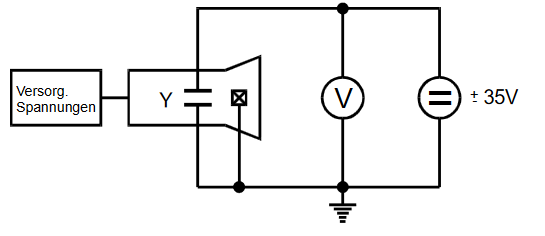
\includegraphics[width=0.7\textwidth]{aufbauE.png}
 \caption{Schaltung für die Unttersuchung der Ablenkung.\cite{sample1}}
 \label{fig:aufbauE}
\end{figure}
Für die Untersuchung der Ablenkung wird die Ablenkspannung hochgeregelt, damit kann der Leuchtfleck
auf neun äquidistante Punkte auf dem Koordinatengitter des Schirms bewegt werden. Die neun zugehörigen
Ablenkspannungen werden notiert, dies geschieht für fünf verschiedene Beschleunigungsspannungen.
\begin{figure}
 \centering
 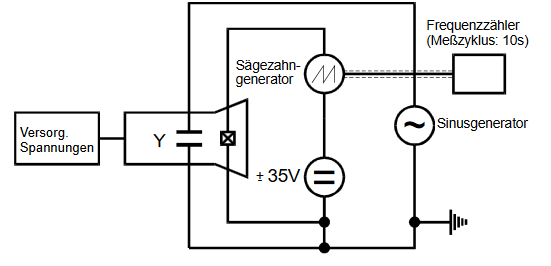
\includegraphics[width=0.7\textwidth]{AufbauO.png}
 \caption{Schaltung für den Oszillographen.\cite{sample1}}
 \label{fig:aufbauO}
\end{figure}
Für den Kathodenstrahl-Oszillographen wird eine Sägezahnspannung in Y-Richtung und eine Sinusspannung
in X-Richtung angelegt. Die Frequenz der Sägezahnspannung wird variiert bis eine stehende Welle auf dem Schirm entsteht
und die entsprechende Sägezahnspannung notiert.
Die geschieht für fünf verschiedene Verhältnisse zwischen Sägezahn- und Sinusspannung.
Ebenfalls wird die Amplitude der stehenden Welle bei konstanter Beschleunigungsspannung vermessen.

Zur Erzeugung des B-Feldes wird eine Helmholz-Spule verwendet. Das Magnetfeld, abhängig vom Strom $I$,
wird senkrecht zum Elektronenstrahl ausgerichtet, welcher in Richtung der zuvor bestimmten Horizontalkomponente
des Erdmagnetfeldes steht. Der Strom $I$ wird hochgeregelt, damit kann der Leuchtfleck auf neun Punkte
auf dem Koordinatengitter des Schirms gelenkt werden. Die zugehörigen Ströme werden notiert.
Diese Messung wird für vier weitere Beschleunigungsspannungen wiederholt.
Zuletzt wird das Erdmagneteld vermessen, indem die Position des Leuchtfleckes vorgemerkt wird
und die Apparatur senkrecht zu der
Horizontalkomponente des Erdmagnetfeldes ausgelegt wird.
Dadurch verschiebt sich die Position des Leuchtfleckes.
Der Strom $I$ wird nun so hochgeregelt bis der Punkt wieder die
Ausgangsposition erreicht.
